\newpage
\section{Hatching}
This project also involves hatching implementation. To accomplish this, C++ and a graphics library named "Cairo" is used.
%\subsection{Introduction}
Basically, Hatching is a pattern of lines and dots that fills an enclosed area. Hatching can be used simply for color. The colors can represent materials or uses in drawings and renderings. There aren't any conventions for use of color in architecture. However, many other disciplines, such as urban planning and cartography, prescribe uses for colors in drawings and maps.
\noindent During the training, I also worked on Hatching. Basically, I have used C++ and a graphics library called Cairo. 
In this project, I've implemented two types of hatching:
\begin{enumerate}
\item Solid fill
\item Pattern fill
\end{enumerate}
\subsection{Solid fill}
\begin{itemize}
\item For Solid Fill, I made a C++ program named "solid.cpp" with help of Cairo graphics library. When it is compiled using:\\
\textit g++ solid.cpp -o output -lcairo
\item Then the executable will be created named "output". Execute it using:\\
\textit ./output
\item Then a file will be created named "hatch.svg" with the given color.
We can simply open it in terminal using command:\\
\textit eog hatch.svg
\begin{figure}[!ht]
\centering
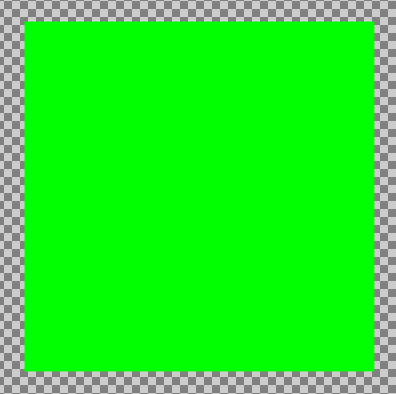
\includegraphics[scale=0.7]{images/hatching/solid.png}                   
\vspace{-1em}
\caption{Solid Fill: hatch.svg}
\hspace{-1.5em}
\end{figure}
\end{itemize}
\subsection{Pattern Fill}
\begin{itemize}
\item For Pattern Filling, I made another program named "pattern.cpp". When it is compiled using:\\
\textit{g++ pattern.cpp -o pexec -lcairo}
\item Then an executable file will be created named "pexec" in the current directory. Execute it using command:\\
\textit{./pexec}
\item Then a file will be created named "hello.png" which contains the hatched object.
Open this file using: \\
\textit{eog hello.png}
%\begin{figure}
%
\includegraphics[scale=0.7]{images/hatching/pattern.png}
%\caption{Pattern Fill: hello.png
%\end{figure}
\begin{figure}[!ht]
\centering

\includegraphics[scale=0.7]{images/hatching/pattern.png}                   
\vspace{-1em}
\caption{Pattern Fill: hello.png}
\hspace{-1.5em}
\end{figure}

\end{itemize}